%
%  emPartAssignment1
%
%  Created by Daniel Beatty on 2012-04-28.
%  Copyright (c) 2012 . All rights reserved.
%
\documentclass[]{article}

% Use utf-8 encoding for foreign characters
\usepackage[utf8]{inputenc}

% Setup for fullpage use
\usepackage{fullpage}

% Uncomment some of the following if you use the features
%
% Running Headers and footers
%\usepackage{fancyhdr}

% Multipart figures
%\usepackage{subfigure}

% More symbols
%\usepackage{amsmath}
%\usepackage{amssymb}
%\usepackage{latexsym}

% Surround parts of graphics with box
\usepackage{boxedminipage}
\usepackage{doublespace}

% Package for including code in the document
\usepackage{listings}

% If you want to generate a toc for each chapter (use with book)
\usepackage{minitoc}

% This is now the recommended way for checking for PDFLaTeX:
\usepackage{ifpdf}

%\newif\ifpdf
%\ifx\pdfoutput\undefined
%\pdffalse % we are not running PDFLaTeX
%\else
%\pdfoutput=1 % we are running PDFLaTeX
%\pdftrue
%\fi

\ifpdf
\usepackage[pdftex]{graphicx}
\else
\usepackage{graphicx}
\fi
\title{An Examination of the Expected Maximization Algorithm Over an Eye}
\author{Daniel D. Beatty  }

\date{2012-04-28}

\begin{document}

\ifpdf
\DeclareGraphicsExtensions{.pdf, .jpg, .tif}
\else
\DeclareGraphicsExtensions{.eps, .jpg}
\fi

\maketitle


\begin{abstract}
\end{abstract}

\section{Specification and Organization} % (fold)
\label{sec:specification}
For the exercise reported here, there is a digital picture of a human retina as shown in figure \ref{fig:8706423-90odl}.  The objective of the work is to 
\begin{enumerate}
	\item Take the gradient of the monochrome image
	\item Use the Expected-Maximization (EM) algorithm to extract the edge points from the blurred optical disc boundary.
\end{enumerate}
\begin{figure}[htbp]
	\centering
		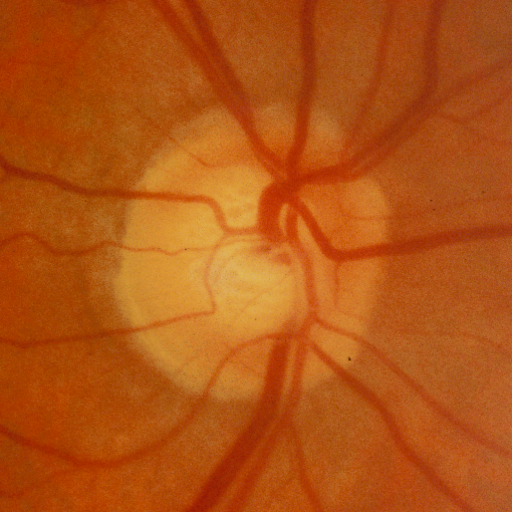
\includegraphics[height=3in]{8706423-90odl.png}
	\caption{Original Image}
	\label{fig:8706423-90odl}
\end{figure}

%You are given a retinal digital picture in color.  Take the gradient of the monochrome image and use the Expectation-Maximization (EM) algorithm to extract the edge points from the blurred optic disc boundary.

% section specification (end)

\section{Background} % (fold)
\label{sec:background}

The expected maximization algorithm is credited as first published in \cite{Dempster77maximumlikelihood}.  Various explanations have appeared in publications like \cite{duda-hart-stork,Moon96theexpectation-maximization, Joo_expectationmaximization}.    

In some explanations, EM extends properties of Maximum Likelihood Estimation (MLE) methods by determining the iterative convergence of sufficient statistics.
\cite{Dempster77maximumlikelihood} showed that the EM algorithm is applied effectively to two datasets.  One data set is observed and the other dataset is realized from the observed dataset.  This application implies that there is a mapping between the two datasets, where as the observed data set itself is deemed incomplete.   The dataset realized from the observed data set is considered a complete dataset.  

In general, the equation for the terminating condition of the EM algorithm \cite{duda-hart-stork} is stated in equation \ref{em_basis}.  
\begin{equation}
\vec{\Theta}^* = \arg \max_{\Theta} \sum_{\vec{x}\in \mathcal{X}^n} E[ \ln p( \vec{x} | \vec{\theta} ,\vec{y}) ] \label{em_basis}
\end{equation}
The meaning of the terms in equation \ref{em_basis} are as follows:

\begin{itemize}
\item  $\mathbf{X}$ is the true data set, $\vec{x}$ is the true data set sample, 
 \item $\vec{\Theta}$ is the set of parameters for the statistic, 
	\item $\vec{\theta}$ is a previous estimate of the set of parameters,  and 
 \item $\vec{y}$ is the data sample in the given data set.
 \end{itemize}

Equation \ref{em_basis} allows a characteristic to be derived in equation \ref{duda-hart-stork-EM} that identifies a convergence point, $Q( \vec{\theta} ; \vec{\theta}^i)$ for the parameters identified by $\vec{\theta}$ and $\vec{\Theta}$,.
\begin{equation}
Q( \vec{\theta} ; \vec{\theta}^i) = E_{D_b} [ \ln p(D_g, D_b; \vec{\theta}) | D_g ; \vec{\theta}^i ] \label{duda-hart-stork-EM}
\end{equation}
where :
\begin{itemize}
	\item $\vec{\theta}^i$ is the current (best) estimate for the full distribution.  
	\item $\vec{\theta}$ is a candidate vector for an improved estimate.
	\item $Q(\vec{\theta} ; \theta^i)$ is a function of $\vec{\theta}$ and $\vec{\theta}^i$.
	\item $D_b$ is the actual data set.  
	\item $D_g$ is the unknown and uncorrupted data set.
	\item $E_{D_b} [ \ln p(D_g, D_b; \vec{\theta}) | D_g ; \vec{\theta}^i ] $ is the expected value over the missing features.  The expected value hinges on $\vec{\theta}^i$ which are the estimated true parameters.
\end{itemize}

 In \cite{yamazaki98introduction}, the complete dataset is assumed to be a collection of Gaussian datasets.   A Gaussian dataset is defined by its mean and variance (or its multivariate equivalent.)  

In the Gaussian case, each class has a proportion that defines how much each class contributes as determined by their mean and covariance (denoted $\alpha, \vec{\mu}, \mathbf{\Sigma}$ respectively).   If one acquires a sample as an initial set, there is an EM algorithm that will find these sufficient statistics. In \cite{yamazaki98introduction}, there is an example using a matrix as the result of the expectation step.  From this expectation, the sufficient statistics for the next step are computed.   When an expected equation forms a matrix $\mathbf{A}$, as in equation 
\ref{expectedMatrix}, it is called an expected matrix.

\begin{equation}
a_{ij}^{(k)}     = \frac {\alpha_j p(\vec{y}_i  ^{(k)}  | \vec{\mu_j} ^{(k)} , \Sigma_j ^{(k)}  )}{\sum_{j=1}^M \alpha_j p(\vec{y}_i  ^{(k)}  | \vec{\mu_j} ^{(k)} , \Sigma_j ^{(k)}  )} \label{expectedMatrix}
\end{equation}


The three sufficient statistics are computed in the maximization step.   They are computed by the following equations.
\begin{eqnarray}
\vec{\mu} _j ^{(k+1)} = \frac{\sum_{i=1} ^N a_{ij}^{(p)} \vec{y}_i} {\sum_{i=1}^N a_{ij} } \label{yamazaki98introduction_Mu} \\
\mathbf{\Sigma} _j ^{(k+1)} = \frac {\sum_{i=1}^N (\vec{y}_i \vec{\mu}_j ^{(p)} )^T(\vec{y}_i \vec{\mu}_j ^{(p)} ) } {\sum_{i=1}^N a^{(k)}_{ij}} \label{yamazaki98introduction_Sigma} \\
\alpha _j ^ {(k+1)} = \frac{1}{N} \sum_{i=1}^N a^{(k)}_{ij}  \label{yamazaki98introduction_proportions}
\end{eqnarray}


As shown in equation \ref{duda-hart-stork-EM}, there is a convergence of probability parameters that can be determined by the $Q$ function, shown in equation \ref{Gaussian-Q}.  
\begin{equation}
Q ( \theta ^* ; \theta ) =\log (\prod_{i=1} ^N  a_{ii} ) \label{Gaussian-Q}
\end{equation}


Also, the initial guess for $\mathbf{A}$ can not be the zero matrix.  As such, the sufficient statistics would be rendered zero, and no convergence would occur.   Typically, the guesses are for $\mu$ to be scattered for each class and for the expected matrix to be 
\[ 
\mathbf{A} = \frac{1}{N} \mathbf{I}.
\]


% subsection demonstrations_of_the_expected_maximization_algorithm (end)

% section background (end)

\section{Approach} % (fold)
\label{sec:approach}

To start, the image is decomposed into a two dimensional array arranged from left to right and top to bottom.   This two dimensional array is then reassembled into a one dimensional array with the following mapping:
\begin{eqnarray}
s[i] = t[x][y] \\
i = y(\bar{r}) + x
\end{eqnarray}
where
\begin{itemize}
	\item $\bar{r}$ is the row size
	\item $y$ is the row index of the pixel, 
	\item $x$ is the column index of the pixel, and 
	\item $i$ is the single dimensional array index of the pixel.
\end{itemize}

The $s[i]$ are thereby considered the observed set and complete set is assumed to be a collection of Gaussian sets.   The number of Gaussian sets is left as a variable.   As in the example given by \cite{yamazaki98introduction}, the complete set is assumed to be a sum of the incomplete set and complete sets.  Thus, a framework is build to compute equations \ref{expectedMatrix}, \ref{yamazaki98introduction_Sigma}, and \ref{yamazaki98introduction_proportions}.  

An Matlab/Octave prototype \footnote{Prototype was authored by Code by Prof. Jose Vicente Manjon Herrera of the Universitat Politècnica de Val{e}ncia} obtains the mean, variance, and proportions from the EM algorithm.   A similar implementation made with the Cocoa Renaissance framework was constructed by the author of this report. % The Cocoa Renaissance framework was first published in the Big Nerd Ranch code fest 2005 as BNRMatrix and BNRWavelet.  

Both algorithms make effective histograms based on the most intense gray level (assuming it is not 1.0).  The Cocoa version produces an 8 bit version to establish the histogram, and performs the remaining computations with the 16 version.   All values are normalize between $[0..1]$.  Both establish a set of parameters for scaling, minimum and maximum values.   The log-likelihood value is determined in both expectation and maximization step for comparison.   If the absolute difference between the two log-likelihood values are within a margin of error, the iteration stops.

\section{Results} % (fold)
\label{sec:results}


The Octave version can not plot images, but the output of vectors from the Octave can be plotted with GNUplot.   The main histogram of the human eye is shown in figure \ref{fig:probability-2}.  This plot shows that the composite image pixel dominance in the low range below 20 and above 50.  In figure \ref{fig:probability}, the results of the EM segmentation is shown.   In this case, one can see the contributions of 5 Gaussian distributions and that combined they almost fit the original.  Also, we can see that certain sections of the image should be distinguishably separated by this filter.


\begin{figure}[htbp]
	\centering
		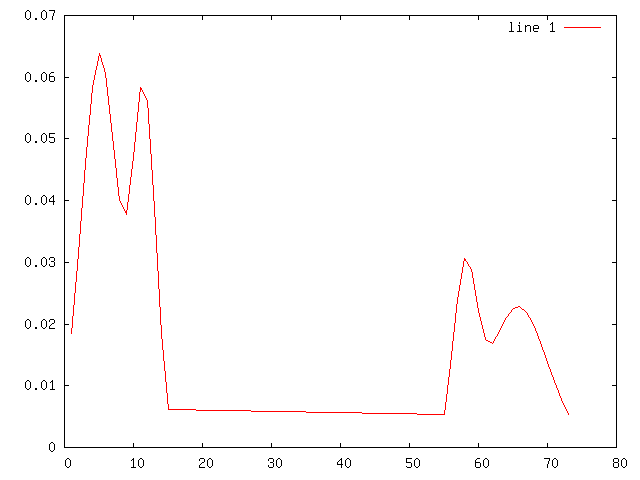
\includegraphics[height=4in]{probability-2.png}
	\caption{Histogram of the Eye image example}
	\label{fig:probability-2}
\end{figure}

\begin{figure}[htbp]
	\centering
		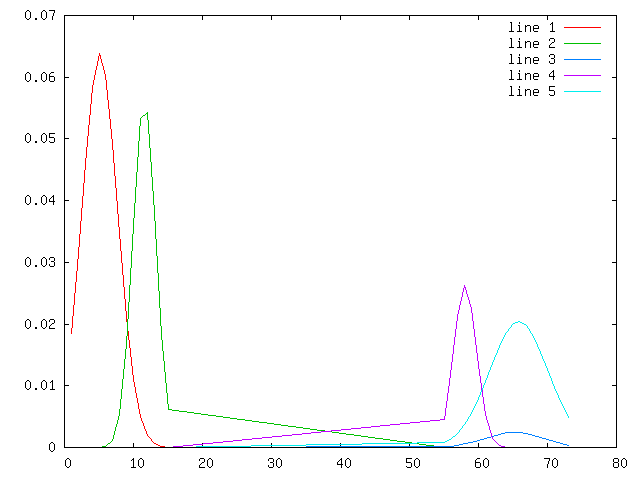
\includegraphics[height=4in]{probability.png}
	\caption{Histogram of the Eye image example with EM Segements}
	\label{fig:probability}
\end{figure}

With the Cocoa implemented version we can the images themselves and play a little the images.  The interface I provided for this program is as shown in \ref{fig:segmentsPanel}.  We can see that the user can select how many Gaussians to apply, and when the computations are performed the sufficient statistics of each Gaussian is listed.  When a sufficient statistic is selected, a filter based on that statistic is applied, as in figure \ref{fig:fiveEmSegments}.  We can see the original image of the eye along with 5 different EM based filters.

\begin{figure}[htbp]
	\centering
		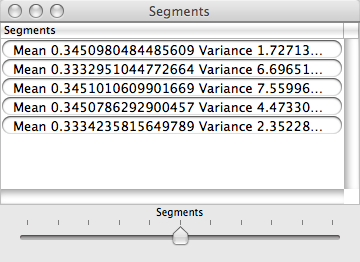
\includegraphics[height=3in]{segmentsPanel.png}
	\caption{EM Segment Control}
	\label{fig:segmentsPanel}
\end{figure}

\begin{figure}[htbp]
	\centering
		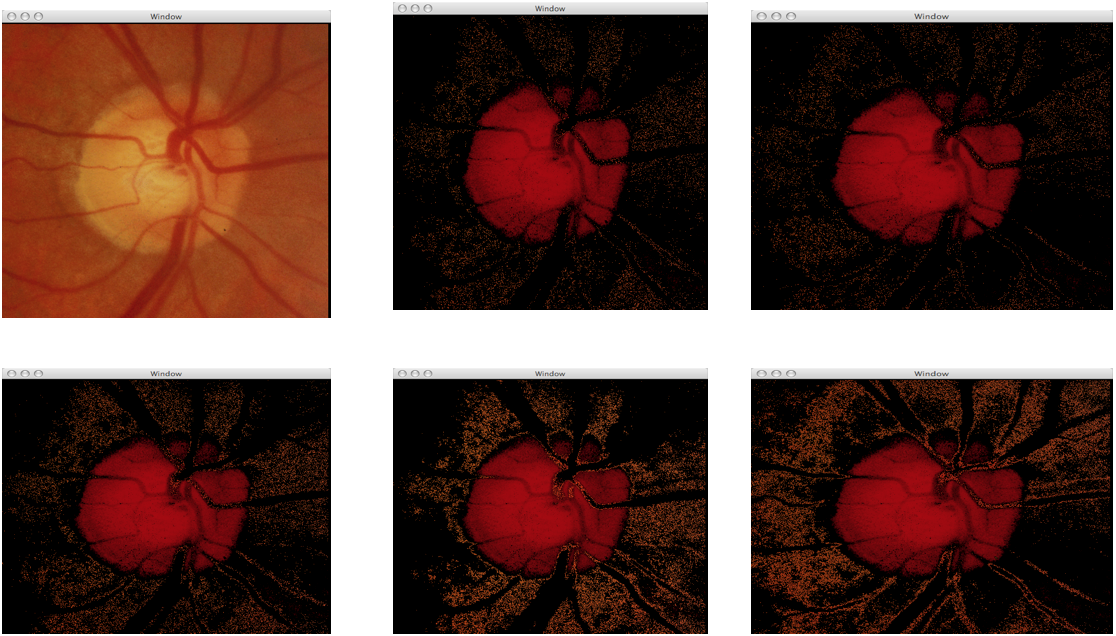
\includegraphics[angle=90,height=8in]{fiveEmSegments.png}
	\caption{Five EM Segments of the Eye and the Original}
	\label{fig:fiveEmSegments}
\end{figure}


% section results (end)

\section{Conclusions} % (fold)
\label{sec:conclusions}

Both iteratively proceed through expectation and maximization step.  The Cocoa version omits adding an $\epsilon$ to the scaled probability calculation, which may be throwing off the Cocoa version by a shift on the x domain.


Also, one filter was difficult to see since does not favor the higher intensity pixels found in the center, and the rest appears dark without that center.

A closer match in the Cocoa version may alleviate some distinction troubles.  Also, a OpenCL plug-in equivalent to other more powerful image editors may be provide a better approach allowing the other filters to be applied to examine the potential of this EM segment filter. 

% section conclusions (end)

\bibliographystyle{unsrt}
\bibliography{../../patternNotes.bib}
\end{document}
